\documentclass{beamer}

\usepackage{tikz}
\usetikzlibrary{shapes.multipart}

\usepackage[dvipsnames]{xcolor}

\usepackage{cite}

%Information to be included in the title page:
\title{Understanding the Structure of District Heating Networks from Measurement Data}
\subtitle{A First Overview}
\author{Fabian Weik}
\institute{Fraunhofer ITWM}
\date{\today}

\begin{document}

\frame{\titlepage}

\begin{frame}
\frametitle{Motivation}
  \begin{itemize}
    \item Sometimes, the information about the structure of district heating networks is incomplete
    \item But needed for precise simulation
      \begin{itemize}
        \item Model does not have to be identical to real network
        \item Rather it should act similarly to the real network
      \end{itemize}
  \end{itemize}
\end{frame}

%\begin{frame}
%\frametitle{Influence of the Structure (Outdated Procedure)}
%  \begin{figure}
%    \begin{tikzpicture}
%      \node (A) [rectangle, draw, rounded corners] at (0, 2) {
%        \begin{tabular}{c}
%          \color{ForestGreen}
%          Inputs \\
%          \color{ForestGreen}
%          Demands \\
%          \color{Orange}
%          Network Structure
%        \end{tabular}
%      };
%      \node (B) [rectangle, draw, rounded corners] at (1, 0) {
%        Flow of Matter
%      };
%      \node (C) [rectangle, draw, rounded corners] at (0, -2) {
%        \begin{tabular}{c}
%          Flow of Heat \\
%          $\Rightarrow$ \color{RoyalBlue} Changing Temperature at Consumers
%        \end{tabular}
%      };
%
%      \draw[->] (A) to [out=310, in=90]  (B) node [midway, right, xshift=30, yshift=20]  {\tiny{affects}};
%      \draw[->] (A) to [out=230, in=135] (C) node [midway, left, xshift=-35]             {\tiny{affects}};
%      \draw[->] (B) to [out=270, in=50]  (C) node [midway, right, xshift=30, yshift=-20] {\tiny{affects}};
%    \end{tikzpicture}
%  \end{figure}
%
%  Computation split for efficiency
%\end{frame}
%

\begin{frame}
\frametitle{Influence of the Structure (Current Procedure)}
  \begin{figure}
    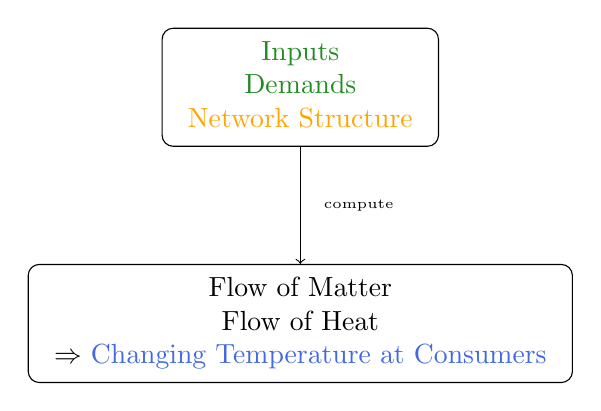
\begin{tikzpicture}
      \node (A) [rectangle, draw, rounded corners] at (0, 1.5) {
        \begin{tabular}{c}
          \color{ForestGreen}
          Inputs \\
          \color{ForestGreen}
          Demands \\
          \color{Orange}
          Network Structure
        \end{tabular}
      };
      \node (B) [rectangle, draw, rounded corners] at (0, -1.5) {
        \begin{tabular}{c}
          Flow of Matter \\
          Flow of Heat \\
          $\Rightarrow$ \color{RoyalBlue} Changing Temperature at Consumers
        \end{tabular}
      };

      \draw[->] (A) to (B) node [midway, right, xshift=5] {\tiny{compute}};
    \end{tikzpicture}
  \end{figure}
\end{frame}

\begin{frame}
\frametitle{Identifying the Structure --- Approach I}
  Somehow compute in the other direction

  \vspace{1em}

  \begin{figure}
    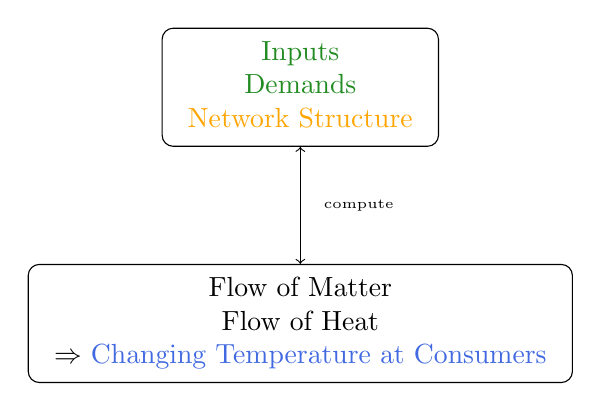
\begin{tikzpicture}
      \node (A) [rectangle, draw, rounded corners] at (0, 1.5) {
        \begin{tabular}{c}
          \color{ForestGreen}
          Inputs \\
          \color{ForestGreen}
          Demands \\
          \color{Orange}
          Network Structure
        \end{tabular}
      };
      \node (B) [rectangle, draw, rounded corners] at (0, -1.5) {
        \begin{tabular}{c}
          Flow of Matter \\
          Flow of Heat \\
          $\Rightarrow$ \color{RoyalBlue} Changing Temperature at Consumers
        \end{tabular}
      };

      \draw[<->] (A) to (B) node [midway, right, xshift=5] {\tiny{compute}};
    \end{tikzpicture}
  \end{figure}

  \vspace{1em}

  Forward computation requires finding loops in the structure.
  This seems very hard to reverse, since not a simple function.
\end{frame}

\begin{frame}
\frametitle{Identifying the Structure --- Approach II}
  Formulate finding the structure as a optimization problem.

  \vspace{2em}

  \begin{itemize}
    \item Possible Connections as parameters
      \begin{itemize}
        \item Single values of edge icidence matrix
        \item Influences loop incidence matrix also
      \end{itemize}
    \item Optimize for low error (discrepancy to measured data)
  \end{itemize}

  \vspace{2em}

  Possibly
  \begin{itemize}
    \item Connections as continuous values instead of discrete
  \end{itemize}
\end{frame}

\begin{frame}
\frametitle{Possible Optimizations for Approach II}
  \begin{itemize}
    \item Use already computed loops to speed up computation of the loops in the new structure
    \item Reducing the problem space:
    \begin{itemize}
      \item Only check connections that make sense
        \begin{itemize}
          \item Based on coordinates
          \item Based on streets
        \end{itemize}
      \item Use heuristics to check most likely first
      \item Group possible connections and disqalify whole groups early
    \end{itemize}
    \item Compute a initial guess with a linear heat/mass transfer model (based on~\cite{wang2024identification})
  \end{itemize}
\end{frame}

\begin{frame}
\frametitle{Measurements and Signals}
  Measurements:
  \begin{itemize}
    \item Temperature and flow at consumers
    \item Flow (Vorlauf) temperature
  \end{itemize}

  \vspace{2em}

  Signals:
  \begin{itemize}
    \item Flow (Vorlauf) temperature
    \item Possibly: flow at consumers
  \end{itemize}
\end{frame}

\begin{frame}
\frametitle{To be Determined}
  \begin{itemize}
    \item Useful signals to send into the network for most helpful data
      \begin{itemize}
        \item Pulse of temperature at producer
        \item Possibly: increse/decrease flow at a consumer
      \end{itemize}
    \item Possibility of inversely computing connections
    \item Possibility of optimizing connections continuously
    \item Possibilities of reducing problem space in case of discrete optimizations
      \vspace{1em}
    \item What other already techniques for identifying the structure of (electrical) networks may apply
  \end{itemize}
\end{frame}

\begin{frame}
\frametitle{References}
  \bibliographystyle{abbr}
  \bibliography{../../../references.bib}
\end{frame}
\end{document}
